\section{A-star search}
\subsection{Basic Idea}

A* is a kind of informed search, which is different from traditional uninformed search (such as bfs). One huge difference is, instead of searching while trying to maintain as least cost as possible in bfs, A* also consider anohter value called heuristic. Figure \ref{astar} is a demostration of A* algorithm. On one hand, the solid line represent the path that we alredy go through, which is an evaluation of the past. On the other hand, the dash line, it represents the estimated/expected cost from current state to the goal, which is an evaluation of the future. 

At every time A* pick the new state with lowest priority from a priority queue. Usually, it considers the past and the future simultaneously. Let's say the priority value is $f$, value of cost is $g$, and heuristic is $h$, then:
$$f = g + h$$

\begin{figure*}[!h]
\centering
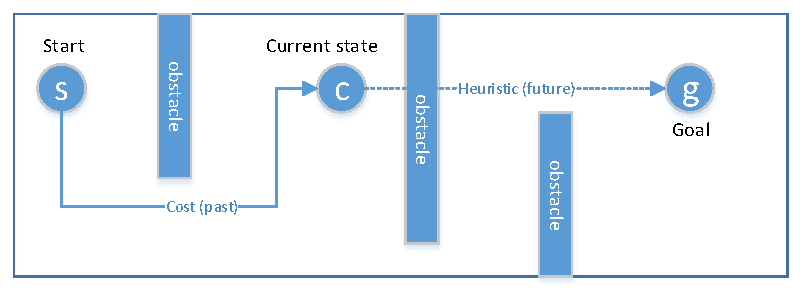
\includegraphics[width=0.927\textwidth]{astar.pdf}
\caption{A demostration of A* algorithm}
\label{astar}
\end{figure*}



\subsection{Code implementation}
\textbf{Line 3-7:} There are three major data structure to help me code astar.
\begin{itemize}
  \item Priority queue: I use a priority queue to store the \emph{frontiers}, sorted by prioirty. Every search I will pop a node from the head of the queue. 
  \item Hash Map $\times 2$: One hashmap maps from node to node, for creating a backchain at the end. Another hashmap maps from node to priority, for the situation when we re-visit a node, it only worth expanding only if it has higher priority/cost than before.
\end{itemize}

\begin{lstlisting}[numbers=left]
public List<SearchNode> astarSearch() {
resetStats();
// implementing priority queue for the frontiers
PriorityQueue<SearchNode> frontiers = new PriorityQueue<>();
// implementing hashmap for the chain and the visited nodes
HashMap<SearchNode, SearchNode> reachedFrom = new HashMap<>();
HashMap<SearchNode, Double> visited = new HashMap<>();

// initiate the visited with startnode
reachedFrom.put(startNode, null);
visited.put(startNode, startNode.priority());
// initiate the frontier
frontiers.add(startNode);
while (!frontiers.isEmpty()) {
  // keep track of resource
  updateMemory(frontiers.size() + reachedFrom.size());
  incrementNodeCount();
  // retrieve from queue
  SearchNode current = frontiers.poll();
  // discard the node if a shorter one is visitedxx
  if (visited.containsKey(current)
	  && visited.get(current) <= current.priority())
	continue;
  // mark the goal
  if (current.goalTest())
	return backchain(current, reachedFrom);
  // keep adding the frontiers and update visited
  ArrayList<SearchNode> successors = current.getSuccessors();
  for (SearchNode n : successors) {
	if (!visited.containsKey(n) || visited.get(n) > n.priority()) {
	  reachedFrom.put(n, current);
	  visited.put(n, n.priority());
	  frontiers.add(n);
	}
  }
}
return null;
}
\end{lstlisting}

\textbf{Line 21-26:} After poping the node, we check for two condition. One is if it is the goal, we simply return the solution path and terminate the search. Antoher condition is, if the node has been visited before, we don't push it into \emph{frontiers} unless it has shorter cost than before.

\textbf{Line 28-36:} Get the successors of currrent node, and push those un-visited nodes or node has shorter cost than before into the \emph{frontiers}.

\subsection{Simple research on cost and heuristic}
A* leverage both the cost (penalty) and the heuristic (search speed). Currently we use $f = h + g$ for priority, which seems quite a balanced solution. What happens if we go to extrem where the priority only related to $g$ or $h$? Or, is 50:50 the best choice for $f$?

Here I modify the expression of priority as following:
$$f = \alpha \cdot h + (1 - \alpha ) \cdot g$$